\chapter{System Development}
\label{chap:sysDevelopent}
This chapter describes development of a multi-vessel platforming system. Major considerations for developing vessel-platform systems that are self-assembling and show collaboration and coordinated motion control as described in Chap. \ref{chap:sysAnalysis} are used for decisionmaking on design and implementation. The multi-vessel-system notation and approach to predict dynamic behavior of a combined waterborne structure as described in Chap. \ref{chap:stateDescription} are used to develop the control algorythm in this chapter. 
The first part of this chapter shows conceptual, high level design choices, such as network topology, control approach and subdivision of the entire system into modular subsystems. 
The second part of this chapter focusses on implementation of the design by giving information of the  technologies, hardware and software structure that give physical form to the distinguished subsystems. 

\section{Design}
\label{sysdesign:Architecture}
The overall design of the control framework is created with the aim to meet the following set criteria.
\begin{itemize}
\item  The system is required to perform automated vessel platform reconfiguration.
\item  The system needs to perform motion control in a collaborative manner, where multiple robots work together to achieve a single goal. 
\item  The system needs to support both above mentioned behaviors simultaneous.
\end{itemize}
Besides hard constraints, several concepts play a key role for making design decisions. 
\begin{itemize}
	\item The framework should support a large amount of-, or arbitrary  configurations.  This creates adaptiveness to a wide set of tasks for modular vessel platforms, which is a key element supporting commercial competitivity.
	\item  Developed solutions are aimed to be general, such that they are applicable or at least meaningful on other ship-systems, environments and scales of operation. This is considered important to stimulate that knowledge gained from the developed experimental setup benefits future commercial implementation.
	\item Solutions are aimed to be modular, such that subsystems are designed to be conveniently swapped out for another (perhaps improved and better performing) version, easing future improvements and increasing reusability of work.
\end{itemize}

The goal of this design is not to optimize an existing system, but to explore a novel combination of behaviors that is expected to be of interest in the near future. 
The ability of succesful assembly needs to be proved, yet successrate and reconfiguration-speed need only be in reasonable limits and magnitude to reflect commercial implementation. Cooperative motion control needs to show convergence of the system to a desired state while a network of robots operate more effective than the sum of individuals, yet quantitiative motion responses need only be stable and within reasonable timeframe. For quantitative performance evaluations (Chap. \ref{chap:evaluation}), criteria are set representing demands of a logistical usecase, shown in Tab. \ref{tab:KPIS}. 

\begin{table}[]
	\centering
	\begin{tabular}{ll}
		Key performance indicator                 & Criteria           \\ \hline
		Risetime*                                 & $t_r$ \textless{}10s      \\
		Settlingtime*                             & $t_s$ \textless{}40s       \\
		Overshoot*                                & ov\textless{}50\%      \\
		Relative motion between connected modules & $\approx 0$      
	\end{tabular}
	\caption{Performance criteria of the designed system. Risetime, Settlingtime and Overshoot pertain criteria for motion control system evaluation, while relative motion between connected modules indicates assembly success. (* evaluated for step inputs 1.0 \& 0.5m translation and 90grad rotation as characteristic motions)}
	\label{tab:KPIS}
\end{table}

Description on design of the experimental setup starts from a high level view by discussing the multi-robot network topology adapting to varying configurations. It continues to explain the general control approach and division in subsystems that each solve a part of the control problem. Design choices of each subsystem are subsequently discussed in terms of model estimation, state estimation, control effort generation, control effort allocation and  assembly protocol. 

\subsection{Fleet Network Topology}
\label{subsection:topologyDesign}
The modules that are used will be rectangular, equipped with two rotating azimuth thrusters. All modules are identical, so a homogeneous fleet is formed. The design has two axes of symmetry, including weight distribution and thruster placement. The origin of the vessel's body fixed coordinate system will be defined where the planes of symmetry coincide. 
The Reseachlab Autonomous Shipping (RAS) Delft has a fleet of such vessels available, named Delfia's (figure \ref{fig:DelfiaOverallLook}). The vessels dimensions are approximately 380 mm long and 200mm wide. The latest version (the Delfia-1* ) is intended to be equipped with a Raspberry-Pi to perform some on board computation tasks whilst also enabling communication via WiFi. 
\begin{figure}[H]
	\centering
	\includegraphics[width=0.9\textwidth]{20210414_121115}
	\caption{Delfia-* vessels, that will act as modules of the fleet system, to perform automated assembly and control.}
	\label{fig:DelfiaOverallLook}
\end{figure}

The approach of dividing a vessel control system via the Guidance, Navigation and Control categorization (\citet{fossen2011handbook} \& section \ref{analysisConfigAdaptation}) is used to distinguish between different system processes. However, the control for this particular system does refer to that of a single vessel, but rather to a set of vessels, which sometimes are controlled individually (when a module moves alone), and in other times together (in assembled platform). Hence, not only the system behavior changes (such as inertia of a platform of variable shape and size), but also the control structure. 


A control structure has been developed, working on three levels, depicted in figure \ref{fig:networkTopology1}. The concept of a 'platform' and a corresponding platform-controller are key to the functioning of this system.  Various tasks of the system are divided across agents that can be roughly described as follows:

\begin{itemize}
	\item A fleet manager
	\item A platform manager
	\item A module
\end{itemize}

\begin{figure}[h]
	\centering
	\includegraphics[width=0.9\textwidth]{networkTopology1V2}
	\caption{Hierarchical topology of the network. A single agent manages various platforms control agents. Platform control agents each manage a unique set of modules.}
	\label{fig:networkTopology1}
\end{figure}

A single fleet manager performs vessel guidance and coordination of the assembly process. These tasks are designed to operate as a rather simplistic state machine that runs trough phases based on system triggers or operator input. 

Tasks generated by the fleet manager are passed onto a set of Platform-controllers, which manage motion control of a set of connected modules in a centralized fashion. For every platform, a single agent is responsible for making decisions for all modules in the platform. This platform controller uses a reference state and a platform-state estimation to generate actuator responses for all modules. These are sent to the corresponding modules that make up the platform, which are then interpreted and executed. The platform controlling agent can be embodied by a computer anywhere on the network, given that it has sufficient computational power and the network is stable and reliable. 

The amount of modules that an platform-control-agent manages varies over time as vessels attach or disconnect. Thus all functions of the platform controller needs to be able to handle a variable amount of modules and configured shape. 

Communication between agents is facilitated by WiFi and the Robotic Operating System (ROS) as middleware. ROS facilitates communication between agents in a multi-robot system in an interoperable and modular way. This is thanks to the publisher-subscriber approach, which allows a variable amount of agents to listen (subscribe) to a dedicated datastream (topic). Similarly, a variable amount of agents can send (publish) various datatypes to such topics. This middleware has several benefits, one of which is the ability to set up various topics that represent some system information, on which agents running on various operating systems can send and receive data. The publisher-subscriber approach allows agents to only be subscribed to topics which are relevant. Furthermore, ROS also has many standardized message formats, libraries, and a large and rapidly developing userbase that further enhances interoperability.

State estimation of modules is done by an on-shore optical tracking system. Each vessel has a dedicated topic on which these estimates are published, which are accessible for all entities within the network by subscribing to that particular topic. 

The fleet manager has, besides creating references for the platforms, also the task of coordinating module ownership. As (dis)assembly criteria are met, platform controllers exchange ownership of a module. This informs a platform-controller that a module is connected, and that it now has access to utilizing that module's actuators. Figure \ref{fig:ownershiptransfer1} and \ref{fig:ownershiptransfer1} illustrate transfer of ownership of a module between two platform controllers, which can leave platform-controller-agents without modules under it's control, rendering it inactive. 
Each module will be controlled by a single platform-controller at a time. The platform controller will have full knowledge of the determined pose of each module in the platform with respect to the platform-coordinate system. 

 \begin{figure}[H]
	\centering
	\makebox[\textwidth][c]{
		\begin{minipage}{0.45\textwidth}
			\centering
			\includegraphics[width=0.95\textwidth]{img/controlAgent_separate}
			\caption{Two vessels that are both controlled by a separate control agent. A change in control structure can transfer module ownership (arrow).}
			\label{fig:ownershiptransfer1}
		\end{minipage}\hfill
		\begin{minipage}{0.45\textwidth}
			\centering
			\includegraphics[width=0.95\textwidth]{img/controlAgent_together}
			\caption{Two vessels that formed into a platform, after which they are both controlled by the same agent.}
			\label{fig:ownershiptransfer2}
		\end{minipage}
	}
\end{figure}

\subsection{Platform Level Control Approach}
\label{subsection:PlatformControlApproach}
The platform controller has the goal of generating and publishing actuator commands for connected modules such that the platform motion follows the reference given by the fleet manager. 
The combined structure formed by the assembling modules will have a changing size and shape . This results in variable platform dynamics and number of available actuators. The overall approach on controlling the platform is illustrated in figure \ref{fig:motionControlApproach}. 
As modules connect or disconnect, the platform controller forms a model of the structure in the new configuration. The approach for estimating this model is elaborated in section \ref{platformModel}. Motion control is based on state feedback, where control effort generation and allocation are separated. The control effort generation block uses the estimated model to adapt actuator behavior to maintain performance while the system dynamics change. 
This control approach considers planar motion in 3-DOF (x, y, and yaw), neglecting pitch, heave and roll. 

\begin{figure}[H]
	\centering
	\captionsetup{justification=centering}
	\includegraphics[width=150mm]{MotionControlAndNavigationLoopV3}
	\caption{The designed platform-motion control loop. State reference $X_{ref}$ is the main input from the Fleet manager (guidance system) and output is vessel state $X$. Occasional changes to configuration are communicated to the platform motion controller for adapting control strategy.}
	\label{fig:motionControlApproach}
\end{figure}

The goal is to find actuator commands for all modules under command of the controller such that the platform state approaches a reference state given by the fleet manager. The reference state will be a position and heading, noted as

\begin{equation}
X_{ref} = \eta_{ref} = \begin{bmatrix} x_{ref}\\ y_{ref} \\ \Psi_{ref} \end{bmatrix}
\label{eqPlatformControlRef}
\end{equation}
which is expressed in $\{n\}$. Note that other approaches might also include velocities as a state that is to be controlled, making the reference, estimated and actual state $X$ a [1x6] vector for motion in the surface plane instead of the [1x3] description as shown in equation \ref{eqPlatformControlRef}.

The control problem is solved in the following steps
\begin{itemize}
	\item An approximate model of the combined body is formed. Control gains are adjusted to estimated model parameters. 
	\item Platform state is estimated
	\item From this model, reference state and estimated state - control efforts are generated by means of a proportional-integrator-derivative (PID) controller.
	\item Control efforts are allocated between actuators on the modules. 
\end{itemize}

The state of the platform is defined as the origin and orientation of platform-body-fixed coordinate system $\{p\}$, expressed as 

\begin{equation}
\eta_{p/n}^{n} = \begin{bmatrix} x_{p/n}^{n}\\ y_{p/n}^{n} \\ \Psi_{p/n}^{n} \end{bmatrix}
\end{equation}

which is expressed in $\{n\}$. Note that platform origin is not defined to coincide with the centre of gravity. Connection of a module to the platform is considered binary, meaning a module would be either connected or disconnected, and cannot be 'connected a little'. Any change in platform configuration would result in an instantaneous displacement of the centre of gravity. As continuity of estimated state is desirable, the use of the centre of gravity was avoided to use as the definition of $\{p\}$.




\subsection{State Estimation}
\label{sec:stateEstimationDesign}

%From a set of sensors (on ships or shore) an estimation of the 'platform state' needs to be made. From this, and information of the modules that make up the platform
The platform state is but a concept to represent a collection of modules and is thus not directly measurable. It is however estimated by using a feedback signal of module positions and their known, constant placement within the body. Signal from a separate system performing state estimation of modules is translated to yield platform state estimates. Module localization can be done on board, on shore and with a variety of sensor systems, yet only needs to be consistently communicated on the robot network. Consider an update of the position and orientation of a module as
\begin{equation}
\eta_{b/n}^{n} = \begin{bmatrix} \textbf{p}_{b/n}^{n} \\[10pt] \Psi_{b/n}\end{bmatrix} = \begin{bmatrix} \textbf{x}_{b/n}^{n} \\[10pt] \textbf{y}_{b/n}^{n} \\[10pt] \Psi_{b/n}\end{bmatrix} 
\end{equation}

The known position of modules with respect to platform coordinate system as described by equation \ref{eq:moduleStaticPlacementEtaDefinition} is used to transform module to platform pose by subsequent rotation and translation. For the three considered degrees of surface plane motion the platform state becomes

\begin{equation}
\eta_{p/n}^{n} = \begin{bmatrix} \textbf{p}_{p/n}^{n} \\[10pt] \Psi_{p/n}\end{bmatrix}
\end{equation}
where
\begin{equation}
 \Psi_{p/n} = \Psi_{b/n} - \Psi_{b/p}
\end{equation}
and
\begin{equation}
\textbf{p}_{p/n}^{n} =  \textbf{p}_{b/n}^{n} - \textbf{p}_{b/p}^{n} =  \textbf{p}_{b/n}^{n} - \textbf{R}(\Psi_{p/n}) \textbf{p}_{b/p}^{p} 
\end{equation}


\subsection{Control Effort Generation}
\label{controlEffortGenerationDesign}
The control block is based on a Proportional-Integrator-Differential (PID) controller, designed to scale to model parameters which are estimated as described in section \ref{platformModel}. Three parralel controllers are used to control each individual degree of freedom, as illustrated in \ref{fig:parralelControl1}

\begin{figure}[H]
	\centering
	\captionsetup{justification=centering}
	\includegraphics[width=0.9\textwidth]{parralelControl1}
	\caption{Parralel controller setup}
	\label{fig:parralelControl1}
\end{figure}

Control gains of the control-effort-generation block are designed to scale such that, once tuned for a single configuration, show similar behavior for any other configuration or platform size. For this, the following configuration dependent parameters are used. \\

\begin{itemize}
	\item Position of the centre of gravity
	\item Linear inertia, or mass
	\item Angular inertia
	\item Maximum available control effort for translation (maximum force)
	\item Maximum available control effort for rotation (maximum torque)
\end{itemize}

The centre of mass of the platform is found using equation \ref{eq:centreOfMassFindR}. It can then be substituted in equation \ref{eq:translatedToPlatformCentreOfMAss2} to express the equations of motion in that particular point. For three degrees of freedom in the surface plane this becomes shaped as

\begin{equation}
	\textbf{M}_{p}^{CG} = \begin{bmatrix}
	m_{xx} 	&	m_{xy}	& 0 		\\[10pt]
	m_{yx} 	&	m_{yy}	& 0 		\\[10pt]
	0 		&	0		& I_{zz} 	\\[10pt]
	\end{bmatrix}
\end{equation}
where

\begin{table}[H]
	\centering
	\begin{tabular}{ll}
		
		$	\textbf{M}_{11} = \begin{bmatrix}
		m_{xx} 	&	m_{xy}	\\[10pt]
		m_{yx} 	&	m_{yy}	\\[10pt] \end{bmatrix}$ & 
		
		$	\textbf{M}_{12} = \begin{bmatrix}	 0 	\\[10pt]  0	\end{bmatrix}$ \\[25pt]
		
		$	\textbf{M}_{12} = \begin{bmatrix}		0 	& 0 \end{bmatrix}$ &
		
		$	\textbf{M}_{22} =  I_{zz} $
	\end{tabular}
\end{table}



Which shows the estimated moment of inertia $I_{zz}$ in the bottomright corner. If modules have hydrodynamic added mass being modelled as a constant, direction-dependent constant, the off-diagonal elements $m_{xy}$ and $m_{yx}$ may be nonzero. This can also result that masses in $xx$ and $ yy$ direction may be unequal, which can feel rather counter intuitive, as this is never the case with normal rigid body motion. The cause of this still originates from the origonal form of module inertia matrix, as this inherited by using such models. 

The controllers responsible for linear motion will use an estimation of the mass of the platform. Rotating the inertial matrix can be done such that the off diagonal elements $m_{xy}$ and $m_{yx}$ become zero. The magnitude of the diagonal elements can be easily found, as they are the eigenvalues of $M_{11}$. The average of the eigenvalues is used as the estimated omni-directional mass for adapting controller behavior. For linear motion in 2 degrees of freedom (x and y) this becomes
\begin{equation}
	m_{p} \approx \frac{1}{2} \sum_{}^{}  Eig ( \textbf{M}_{11} )
\end{equation}

As the fleet utilizes rotatable azimuth thrusters, the maximum force is generated by the propellers on full power in a single direction. The maximum force that the platform can generate can be found by summation of maximum thruster force of all thrusters
\begin{equation}
\textbf{f}_{p,max} = \sum_{i=1}^{n_{thr}} f_{i,max}
\end{equation}
where $n_{thr}$ refers to the total amount of thrusters, and $f_{i,max}$ is the maximum force that the $i$th propeller can supply. The homogeneous fleet has two identical propellers per module, such that. 
\begin{equation}
\textbf{f}_{p,max} = 2*n* f_{prop,max}
\label{Maxforce1}
\end{equation}

Maximum torque is generated when all thrusters supply maximum force in the direction perpendicular to a vector between CG and the thruster. For a single vessel, this becomes
\begin{equation}
\textbf{m}_{i,max} = |\textbf{r}|  f_{i,max} =  | \textbf{p}_{CG/p}^{p} - \textbf{p}_{thr,i/p}^{p} |  f_{i,max}
\label{maxMoment1}
\end{equation}
where $ \textbf{p}_{CG/p}^{p} $ is the position vector of the platform $CG$ and $ \textbf{p}_{thr,i/p}^{p}$ is the position of the $i$th thruster. The latter is usually given in local frame of a module, but can be converted to platform coordinates by matrix rotation and a translation as:
\begin{equation}
\textbf{p}_{thr,i/p}^{p} =   \textbf{R}_{bj}^{p} \textbf{p}_{thr,i/bj}^{bj} + \textbf{p}_{bj/p}^{p}
\end{equation}
where $\textbf{p}_{thr,i/bj}^{bj}$ is the position of thruster $i$, mounted on module $j$, expressed in the body fixed coordinate system of module $j$. $\textbf{p}_{bj/p}^{p}$ is the position of module $j$ expressed in platform coordinate system. Summation of equation \ref{maxMoment1} over all modules yields total maximum torque generated by actuators for a given configuration as

\begin{equation}
\textbf{m}_{p,max} = \sum_{i=1}^{2n}  \textbf{m}_{i,max}
\label{maxmomentTotalSummed}
\end{equation}

It should be noted that the  equation \ref{Maxforce1} and \ref{maxmomentTotalSummed} show absolute maxima, which need full participation of all actuators to be reached. These maxima can not be obtained in different degrees of motion simultaneously, as outputs will be saturated. To avoid unpredictable control effort generation, actuator operation near output saturation is avoided during implementation.

The control blocks for each degree of freedom, as shown in figure \ref{fig:parralelControl1} operate based on PID control. Generic PID control starts by computing the state error by taking the difference between reference and state feedback. This error is fed parralel trough three different gains, where one signal is integrated and one is differentiated, until the signals are summed to yield the control output.

\begin{figure}[H]
	\centering
	\captionsetup{justification=centering}
	\includegraphics[width=0.4\textwidth]{simplePIDGeneric}
	\caption{A generic Proportional-Integral-Derivative control structure.}
	\label{fig:simplePIDGeneric}
\end{figure}

The control gains of the three parralel PID controllers are tuned to a single reference configuration. As the configuration changes the control gains will adapt to the newly estimated dynamics. 
The control gain scaling is based on the assumption that a configuration will have a response comparable to the reference, but in a different time scale. Typical errors that are fed into PID gains will thus be of comparable magnitude. System responses of current and reference configurations are thus aimed to be approximately comparable such that
\begin{equation}
	\eta_{c}(t) \approx \eta_{ref}(C*t)
	\label{eq:timescaling}
\end{equation}


 If control forces are a dominant factor to the response time of a step input on the system, a characteristic accelleration of a configuration can be defined as
\begin{equation}
a = \frac{Force}{Inertia}
\end{equation}

This is used to estimate the time scaling factor is estimated as the ratio of maximum accelleration of a configuration with respect to the reference configuration. 
\begin{equation}
C_{c} = \frac{a_{c}}{a_{ref}} = \frac{F_{c} \; I_{ref}}{F_{ref} \; I_{c}}
\label{eq:timescaleDef}
\end{equation}
where $ a_{c}$ and $a_{ref}$ are the characteristic accellerations of the current and reference configuration respectively. 

All gains is designed to scale to the maximum obtainable control effort. The base value of contribution is determined in the gain tuning process of the reference configuration. The eventual output of any proportional integral and derivative gains is multiplied by the maximum control effort in that dimention. 

Output of the control effort from proportional gain scales to the magnitude of the error, which assumed comparable in all configurations.  This could result in, for example, a proportional gain that is to contribute 60\% of the maximum obtainable control effort at an error of $e = 1.0$. The gain would become 
\begin{equation}
	K_{p} = K_{p,base}* \tau_{max} =  0.6* \tau_{max}
\end{equation}
such that the control effort contributed by the proportional block becomes
\begin{equation}
	\tau_{i,prop} = e * K_{p} = 0.6* \tau_{max}
\end{equation}

Integral control is however affected by the time in which the system responds. A system that responds slower ( $C_{c} < 1$ ) than the reference configuration will encounter additional integrator buildup. Time factor $C_{c}$ compensates for change of integrator output due to response time by adjusting integral gain as
\begin{equation}
	K_{i} = C_{c} \; K_{p,base} \; \tau_{max}	
\end{equation} 
such that integral control output becomes
\begin{equation}
\tau_{i,int} =  K_{i} \int_{0}^{t} e \; dt =  C_{c} \; K_{p,base} \; \tau_{max} \int_{0}^{t} e dt
\end{equation}

Derivative control output is also affected by time, but scales inversely to time factor $C_{c}$ with respect to integral control. Imagine, for example, a mass (*cough* *cough* vessel) that approaches the reference state, which would make the time derivative of the error negative. Derivative control would attempt to slow the mass down as it approaches it's desired state to avoid overshoot. An object, such as a container vessel, with low maximum control forces relative to the large mass would have to use take this speed more serious than highly manouverable vessels. Derivative adapts to a configuration as
\begin{equation}
K_{i} = \frac{K_{d,base} \; \tau_{max}}{C_{c}}	
\end{equation} 

Base values of controller gains ( $K_{p,base}$ ,$K_{i,base}$ ,$K_{b,base}$ ) will be set while revieuwing responses of the system in reference configuration. A PID controller can be manually tuned, or with the help of many tools such as automated PID tuning software. Linear motion in $x$ and $y$ direction will have identical control settings, as dependency on the orientation of reference frame $\{n\}$ is considered undesirable. 

\subsection{Control Effort Allocation}
\label{controlEffortAllocationDesign}
Control effort, as shown in the previous section, needs to be allocated onto the platform's actuators. The amount of thrusters available varies per configuration. Also placement and orientation of actuators can differ. 
A platform needs to be able to sufficiently control it's motion in all reasonably forseeable configurations. As the amount of different configurations is rather large, a general solution is used, that can solve the control effort allocation problem for all possible configurations. 
The designed control effort allocation protocol relies on the following main principle:
"The contribution of an actuator to a desired resulting force or moment is proportional to   its ability to contribute relative to that of the combined set of actuators."

This principle manifests particularly in rotational motion, as the ability of a thruster to generate torque relies on its placement with respect to the centre of gravity. Linear motion turns out not to exhibit such dependencies, as all thrusters are equal in strength, and possible orientation.  To compute actuator commands that satisfy the desired control effort,
it is allocated in each degree of freedom individually and finally combined.

Position of a thruster with respect to $CG$ can be expressed in $\{p\}$ by
\begin{equation}
\begin{split}
\textbf{p}_{t/CG}^{p} = \textbf{p}_{t/b}^{p} + \textbf{p}_{b/p}^{p} - \textbf{p}_{CG/p}^{p} \\
= \textbf{R}_{b}^{p} \textbf{p}_{t/b}^{p} + \textbf{p}_{b/p}^{p} - \textbf{p}_{CG/p}^{p}
\end{split}
\end{equation}

Thruster force vector can be expressed in $\{p\}$ in 3 degrees of freedom as
\begin{equation}
\begin{split}
\textbf{f}_{t}^{p} = \textbf{R}_{b}^{p} \textbf{f}_{t}^{p}
\end{split}
\end{equation}

The total resultant control effort from all modules in the centre of mass can be found by
\begin{equation}
m_{CG} = \sum_{i =1}^{n_{thrusters}} \textbf{p}_{ti/cg} \times \textbf{f}_{ti}
\label{torqueCG1}
\end{equation}
\begin{equation}
f_{CG} = \sum_{i =1}^{n_{thrusters}}  \textbf{f}_{ti}
\end{equation}
or in vector form as
\begin{equation}
\tau_{CG} = \sum_{i =1}^{n_{thrusters}}  \textbf{H}^{\top}(\textbf{p}_{t/CG}^{p}) \begin{bmatrix}
\textbf{f}_{ti}^{p} \\ 0_{1x3}
\end{bmatrix}
\end{equation}
where $\textbf{p}_{ti/CG}$ is the position of the $i$th thruster with respect to the platform's centre of gravity, and $\textbf{f}_{ti}$ refers to the force vector applied by the $i$th thruster.
Where it should be noticed that the zeros represent torque applied by the propeller, as propellers are modelled as a forcevector applied in a point. A resulting moment can be created due to the fact that thrusters are placed at a distance from $CG$.


The approach on generating control effort that results into torque is as follows. A force at a distance from $CG$ creates a higher resulting torque. The linear relation between torque and distance between applied point and $CG$ can be seen in equation \ref{torqueCG1}. Only considering forces in the $xy$ plane gives
\begin{equation}
	m_{zz} = x_{ti/CG} \; f_{y}  \; -  y_{ti/CG} \; f_{x}
	\label{mzz3dof}
\end{equation}
So at a constant force, the generated moment proportionally increases with distance. For a single direction ($x$ or $y$) this would be shaped as shown in figure \ref{fig:rampThrust}. Thruster contibution to torque that is to be deployed proportional to the effectiveness of the thruster results in a quadratic shape. Figure \ref{fig:paraThrust} shows how the quadratic contribution of a thruster at varying distance

\begin{figure}[H]
	\centering
	\makebox[\textwidth][c]{
		\begin{minipage}{0.45\textwidth}
			\centering
			\includegraphics[width=0.95\textwidth]{ThrustAllocPara}
			\caption{Linear relation between resulting moment and thruster distance from $CG$, while thruster force is constant}
			\label{fig:rampThrust}
		\end{minipage}\hfill
		\begin{minipage}{0.45\textwidth}
			\centering
			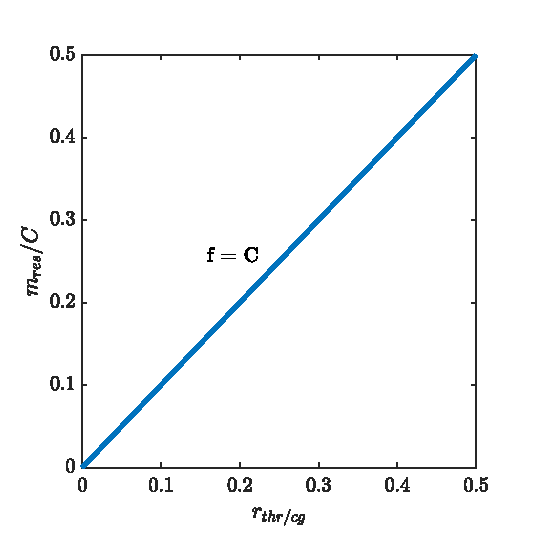
\includegraphics[width=0.95\textwidth]{ThrustAllocLin}
			\caption{Quadratic relation between resulting moment and thruster distance from $CG$, due to a thruster force being controlled to be proportional to distance}
			\label{fig:paraThrust}
		\end{minipage}
	}
\end{figure}

Thruster force to contribute to realizing a desired resulting moment is set as
\begin{equation}
	f_{x} = C_{m} \; m_{d} \; (- y_{ti/CG})
	\label{fx1}
\end{equation}
\begin{equation}
	f_{y} = C_{m} \; m_{d} \; x_{ti/CG}
	\label{fy1}
\end{equation}
where $C_{m}$ is a configuration dependent participation factor for torque and $m_{d}$ is the desired resulting moment of the combined structure. The resulting moment of a thruster becomes (by substituting \ref{fx1} and \ref{fy1} in \ref{mzz3dof})
\begin{equation}
m_{ti} = C_{m} \; m_{d} \; [ x{_{ti/CG}}^{2} \; + \; y{_{ti/CG}}^{2} ]
\end{equation}
The resulting moment of all thrusters satisfies
\begin{equation}
\begin{split}
m_{res} = m_{d} =  \sum_{i =1}^{n_{thrusters}} m_{ti} \\
= C_{m} \; m_{d} \; \sum_{i =1}^{n_{thrusters}}  \; [ x{_{ti/CG}}^{2} \; + \; y{_{ti/CG}}^{2} ]
\end{split}
\end{equation}
From which the total configuration dependent participation factor can be found, as
\begin{equation}
\begin{split}
C_{m} = \frac{1}{ \sum_{i =1}^{n_{thrusters}}  \; [ x{_{ti/CG}}^{2} \; + \; y{_{ti/CG}}^{2} ] }
\end{split}
\end{equation}
This constant ends up scaling all thruster contribution such that the overall relationship between thruster contribution and distance is quadratic, and that the resultant moment matches the desired moment. 


For linear motion a similar principle of contribution to effectiveness is applied, yet turns out much simpler. The homogeneous fleet has thrusters that are all equal in strength, and able to turn in all directions. As all thrusters are thus equally able to contribute to linear motion, total desired thrust is equally divided between all thrusters such that

\begin{equation}
f_{d} = \sum_{i=1}^{n_{thrusters}} * f_{ti}
\end{equation}

\begin{equation}
f_{ti} = C_{f} \; f_{d}\;  f_{max}
\end{equation}

\begin{equation}
C_{f} = \frac{1}{n_{thrusters}}
\end{equation}


All degrees of freedom that are affected by elements from the vector of desired control effort are evaluated independently, resulting in a forcevector for every thruster for every degree of freedom. The forcevectors pertaining to a thruster in all degrees of freedom are summed to obtain the overall contribution of that thruster. For three degrees of freedom this becomes
\begin{equation}
	\textbf{f}_{ti} = \textbf{f}_{ti,fx} + \textbf{f}_{ti,fy} + \textbf{f}_{ti,m}
\end{equation}
Fig. \ref{fig:controlAllocationSeparate1} illustrates how the control allocation problem is solved by combining actuator responses from elements of the desired control effort vector. 

\begin{figure}[H]
\centering
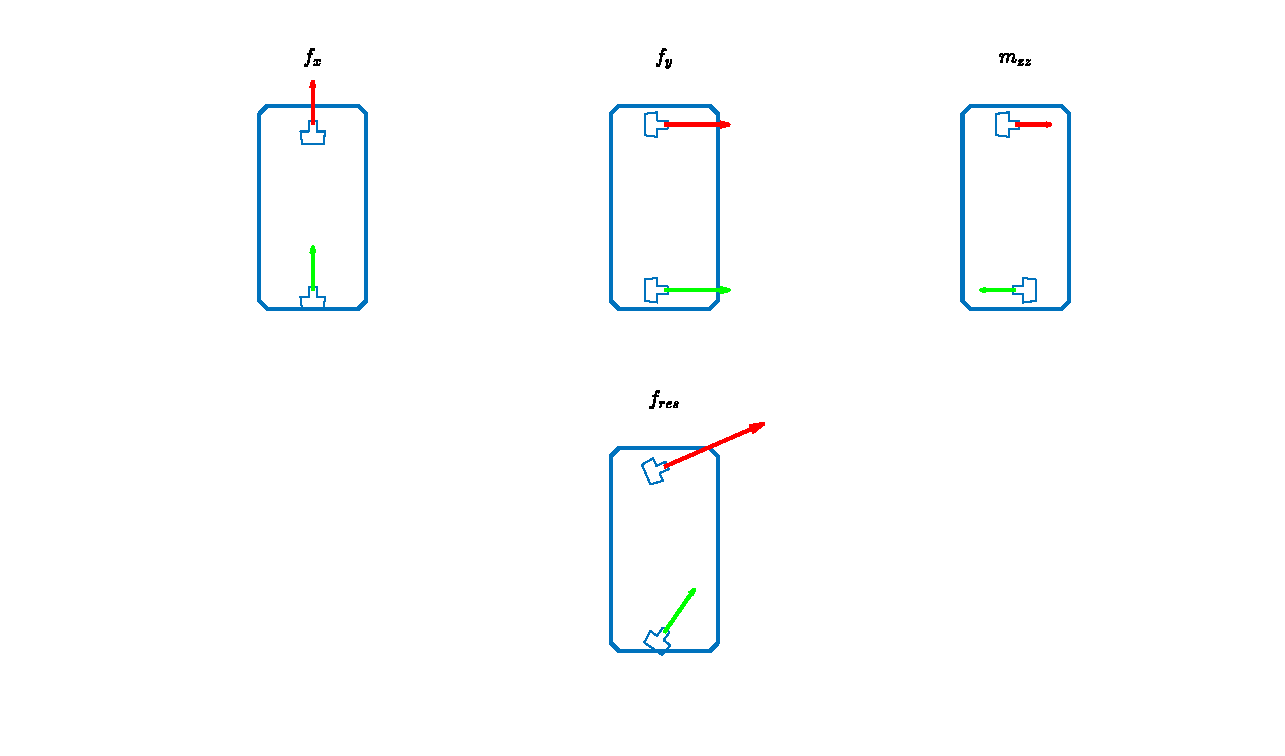
\includegraphics[width=\textwidth]{actuation_combined}
\caption{The approach of solving control allocation in each dimention separately, illustrated for a single vessel configuration. Three dimensions along which control effort is required are solved (above). The forces of the three solutions are combined to yield the final solution (below). }
\label{fig:controlAllocationSeparate1}
\end{figure}

\subsection{Assembly Protocol}
\label{assemblyProtocolDesign}
Modules will assemble in a lattice structure, using active magnets to remain configured. Task execution, including assembly, operates in a phasewise fashion. Generating the desired configuration (blueprint) and assembly planning are done by the operator for this project. 
The following steps are considered to achieve assembly of a module or platform to another:
\begin{itemize}
	\item The connecting object lines up with the assembly at a short distance, such that it can freely reach the connection site. During this process both objects are controlled by different controllers. 
	\item The connecting object moves to the connection site. Magnet connectors within area of acceptance of a connection site make contact, and connect. 
	\item Success of connectivity is evaluated before continuing
	\item If connected, ownership of the connecting bodies is transferred to the controller of the assembly. The other controller becomes inactive. (see figure \ref{fig:ownershiptransfer1} and \ref{fig:ownershiptransfer2})
	\item The controller of the assembly recomputes configuration dependent parameters on:
	\begin{itemize}
		\item The estimated platform model, as in section \ref{platformModel}
		\item The control effort generation protocol, by adapting controller gains to the newfound model estimate, as in section \ref{controlEffortGenerationDesign}
		\item   The control allocation protocol, to divide generated control effort over the new configuration as described in section \ref{controlEffortAllocationDesign}.
	\end{itemize}
	\item The assembly runs the adapted control scheme for further tasks.
\end{itemize}


\begin{figure}[H]
	\centering
	\includegraphics[width=0.7\textwidth]{matlabEvaluationFig14c}
	\caption{Platform assembly protocol from top vieuw. Vessel 1 and 3 are lined up to approach connecting to vessel 2 on either side. Once connectors are within range, the magnets snap into place, fixing relative motion.}
	\label{fig:matlabEvaluationFig14c}
\end{figure}


% The forces and moments represented by the acceleration hydrodynamic coefficients can, to a very great extent, be modeled as potential flow phenomena. Neglecting the details of the boundary layer in modeling acceleration-dependent forces and moments acting on a submerged body yields quite satisfactory results for most stability and control simulation. " \ref{humphreys1978prediction}


	
\section{Implementation} %Control Approach}
\label{chap:controlApproach}

The conceptual design elements that are explained in the previous section have been implemented to represent the envisioned framework. This section illustrates how designed concepts are realized in various hardware and software components. 

Physical system components are first introduced to shed light on the experimental facility, localization system and give more details on low level actuator control systems running on the modules. The multi-robot network setup is explained showing how various system components communicate. A object oriented Matlab software-framework been developed aimed to be reusable and intererable for other multi-vessel experiments within RAS. This framework, its structure, relation between classes, and means of implementing the designed control approach are explained in section \ref{sec:controlSoftware}.

Throughout developments many iterative changes were made to the system, of which two facets are discussed in section \ref{AdjustmentsAfterTests} starting with the process of tuning control gains and secondly an improvement of the assembly protocol using normal forces between modules to aid connectors reaching area of acceptance. 

Behaviors and responses of the system in development are occasionaly shown to support design choices. Behavior of the system in final stage of development is shown and evaluated in the next chapter. 

\subsection{System Components}
\label{imp:syscomponents}
The implemented control system consists of three key components
\begin{itemize}
	\item An optical tracking system for module localization.
	\item A computer that executes the control protocol and distributes generated tasks to the entire fleet.
	\item A set of Delfia-1* modules
\end{itemize}

This section provides details on the experimental setup of the optical tracking system and modules. Functionality of the control software is discussed in a separate section (\ref{sec:controlSoftware}). 

%\subsubsection{Experimental facility and Optical tracking system}
The experimental setup is designed to operate in the towing tank facility of section Maritime and Transport Technology (section MTT) in the faculty of Mechanical, Maritime and Materials Engineering (Faculty 3ME). One of such tanks is equipped with an optical sensing and interpretation system from the brand Optitrack. A 40 meter section of the tank is covered by cameras. Optitrack's motion capture software supports defining a set of infra-red reflectors as a rigid body. The camera setup was set up to interpret images to estimate state of the defined bodies (modules), and broadcast them on dedicated ROS topics at a frequency of 30hz. 

\begin{figure}[h!]
	\centering
	\captionsetup{justification=centering}
	\includegraphics[width=0.9\textwidth]{img/IMG_4805b_downsized}
	\caption{The MTT towing tank facility at 3ME.}
\end{figure}


\begin{figure}[H]
	\centering
	\makebox[\textwidth][c]{
		\begin{minipage}{0.4\textwidth}
			\centering
			\includegraphics[width=0.95\textwidth]{img/singleDelfiaInfraRedTrackers}
			\caption{Five infra-red reflectors on top of a Delfia-1* module.}
		\end{minipage}\hfill
		\begin{minipage}{0.55\textwidth}
			\centering
			\includegraphics[width=0.95\textwidth]{img/IMG_4810_downsized}
			\caption{Motion tracking cameras mounted along the experimental setup.}
		\end{minipage}
	}
\end{figure}

\begin{figure}[H]
	\centering
	\includegraphics[width=0.7\textwidth]{OptitrackRays}
	\caption{Optitrack motion tracking with the towing tank setup, showing two deployed vessels. Green lines depict rays of reflectors that are succesfully being tracked}
\end{figure}


%\subsubsection{Delfia-1* Modules}
The Delfia-1* vessel (also refferd to as 'Delfia') is a model scale, electrically powered ship, equipped with two 360 degree rotatable azimuth thrusters. There are a total of four main actuators that are controlled by an on board system, referred to as the 'low-level control system'. The two azimuth thrusters are identical, and both have their orientation and propeller speed managed by a single microprocessor of the open-source Arduino project. Control of propeller speed and thruster angle is done with different hardware components, yet both rely on similar PID feedback control principles. Figure \ref{DelfiaDOF} illustrates the states that the low level control system needs to manage for one thruster. 

\begin{figure}[h!]
	\centering
	\includegraphics[width=0.7\textwidth]{IMG_4564}
	\caption{Degrees of freedom of one azimuth thruster. Each thruster (front and back) needs its direction (red) and propeller speed (blue) controlled.}
	\label{DelfiaDOF}
\end{figure}
All decisions for the low level control system are made on the on board microprocessor. This controller responds to actuator reference commands via USB serial port connection. Connectivity of the low level control system with other elements in the network is done through a Raspberry-Pi, as illustrated in figure \ref{delfiaConnectionNW}. The Raspberry-pi is the connecting element to the ROS network (via wifi) and the Arduino (via USB serial protocol). Other solutions exist that provide similar connectivity, yet a Raspberry-pi has some processing power which allows distribution of some, or all control tasks in future projects. 

\begin{figure}[H]
	\centering
	\includegraphics[width=0.5\textwidth]{DelfiaNetworkSchematicLowLvl1}
	\caption{The interaction of the Delfia's low level control system with on board computer (Raspberry-pi) and the vessel network.}
	\label{delfiaConnectionNW}
\end{figure}

The propeller is powered with an electrical 12V DC engine, while a sensor signal on speed is created by means of an optical encoder. Figure \ref{DelfiaDriveTrain} shows the propeller drivetrain that can be found above each thruster, and figure \ref{propellerFBLoop} illustrates the feedback loop that controls propeller velocity. 

 \begin{figure}[h!]
	\centering
	\makebox[\textwidth][c]{
		\begin{minipage}{0.45\textwidth}
			\centering
			\includegraphics[width=0.95\textwidth]{img/delfiaDriveTrain_edited}
			\caption{The propeller drivetrain. The rotation in the axle of the DC-motor is transferred to the propeller via a belt and gears.}
			\label{DelfiaDriveTrain}
		\end{minipage}\hfill
		\begin{minipage}{0.45\textwidth}
			\centering
			\includegraphics[width=1.1\textwidth]{img/propellerFBLoop}
			\caption{The feedback loop of the low level propeller-speed control system}
			\label{propellerFBLoop}
		\end{minipage}
	}
\end{figure}

Each thruster angle is actuated by a ''Parallax Feedback 360° High-Speed Servo''. Thruster and servo are connected via a rubber cog belt (figure \ref{DelfiaServoTrain}). The servo needs a 50Hz PWM signal as input and uses a hall effect sensor to provide angular position feedback as a 910Hz PWM signal. The feedback loop that controls the thruster angles is as shown in figure \ref{DelfiaServoLoop}.

 \begin{figure}[h!]
	\centering
	\makebox[\textwidth][c]{
		\begin{minipage}{0.45\textwidth}
			\centering
			\includegraphics[width=0.95\textwidth]{img/delfiaServo_edited}
			\caption{The propeller drivetrain. The rotation in the axle of the DC-motor is transferred to the propeller via a belt and gears.}
			\label{DelfiaServoTrain}
		\end{minipage}\hfill
		\begin{minipage}{0.45\textwidth}
			\centering
			\includegraphics[width=1.1\textwidth]{img/servoFBLoop}
			\caption{The feedback loop of the low level thruster angle control system}
			\label{DelfiaServoLoop}
		\end{minipage}
	}
\end{figure}


Fundamentals of the Delfia-1* low level control system have been developed during a research project \citet{boogmans2020Delfia}, by the same author as this work. Development of hardware and software is described therein, and parameter tuning is done by means of evaluating reference step responses. Characteristic control system behavior is shown in figures \ref{delfiaLowStepProp1} and \ref{delfiaLowStepServ1} for propeller-speed and thruster-angle respectively. Note how the propeller speed signal contains significant fluctuations, of which the majority is considered sensor noise. An optimum trade-off point of signal filtering was found between smoothness and increased latency. High frequency notes in this signal (order of $10^3$hz) that translate to engine control effort will not result in noticable differences of vessel dynamics response, as the  vessel responds in much lower frequencies (order of $10^0$ hz). 

\begin{figure}[H]
	\centering
	\includegraphics[width=0.85\textwidth]{img/4e-2_2e-2_0_130hz_n=8}
	\caption{Measured signal of a characteristic step-response of the propeller-speed control system. Considerable high frequency notes can be observed, although it oscillates rather well around the reference input.}
	\label{delfiaLowStepProp1}
\end{figure}

\begin{figure}[H]
	\centering
	\includegraphics[width=0.85\textwidth]{img/Kp_1e0_Ki_8e-3_Kd_4}
	\caption{Measured signal of a characteristic step-response of the thruster-angle control system.}
	\label{delfiaLowStepServ1}
\end{figure}

It is worth noting that the slope of the servo step response, as shown in figure \ref{delfiaLowStepServ1}, proved quite consistent with more agressive controller gains. Higher proportional or integral gain caused more overshoot, or even instability, without the benefit of a quicker response time. This is considered simply due to the maximum rotation speed of the servo. 


Actuators that connect the modules have been developed and implemented as a set of active magnets, or solenoids, shown in figure \ref{fig:solenoidsMF} and \ref{fig:solenoids}. Models are available in various lifting capacities, and a $10N$ model that operates at $12V$ was estimated to provide enough force for vessels to remain connected in reasonably expected scenarios. It is powered by the $12V$ micro powergrid from the on-board battery.  Higher powered magnets draw more power, and this variant seemed a good balance at a $1.0W$ power consumption. Mounts for the connectors were developed and fabricated by a 3D printer to fit in existing slots in the Delfia's hull.

At first, connections were implemented where a connection was made between two vessels with connectors of opposite polarity. Magnet connector polarity can be reversed by reversing the potential on coil connectors. This can be automated with, for instance, an H-bridge. Tests proved connector force to be insufficient between connecting solenoids. Attracting forces to a piece of iron did give the desired results, thus connector counterparts were lathed to size. Available 3D printers proved to have tolerances sufficient such that connector parts, both magnet and piece of iron, were made to stay in the mouts by using a press. 


 \begin{figure}[H]
	\centering
	\makebox[\textwidth][c]{
		\begin{minipage}{0.48\textwidth}
			\centering
			\includegraphics[width=0.95\textwidth]{img/IMG_4812_downsized}
			\caption{An active (right) and passive (left) magnetic connector in a (white) 3D-printed hull mount.}
			\label{fig:solenoidsMF}
		\end{minipage}\hfill
		\begin{minipage}{0.48\textwidth}
			\centering
			\includegraphics[width=0.95\textwidth]{IMG_4814_downsized}
			\caption{Active magnet mounted in the hull of a Delfia-1* module to connect modules into a rigid platform.}
			\label{fig:solenoids}
		\end{minipage}
	}
\end{figure}

\subsection{Network setup}
The backbone of the communication system is deployment of ROS over an internet network. Vessels connect over WiFi, while shore facilities connect to the network router through ethernet cables. ROS provides various standardized messagetypes to improve interoperability and modularity. Various conventions that are developed throughout this project are intended to serve as a framework for further development and reasearch in the facilities of Researchlab Autonomous Shipping. The proposed standardization includes:
\begin{itemize}
	\item ROS message types for control related signals
	\item Naming convention for control related ROS-topics
	\item IP adress reservations for vessels and other components
\end{itemize}
Table \ref{tab:ROSmsgTypeTable} shows the proposed conventions for communication over ROS in RAS facilities. 

\begin{table}[H]
	\centering
	\begin{tabular}{lll}
	Topic content & Messagetype & Naming convention \\[10pt] \hline
	Vessel position and orientation	&$geometry\_msgs/PoseStamped$ &  $/vrpn\_client\_node/<vesselname>/pose$    \\[10pt]
	
	Vessel Actuation	&   $std\_msgs/Float64MultiArray$     & $/actuation<vesselname>$  \\[10pt]
	
	\begin{tabular}[c]{@{}l@{}} Controller reference (for surface \\ plane dynamic positioning systems) \end{tabular} & $ geometry\_msgs/Pose2D$ &   $ /reference<controllername> $
	\end{tabular}
	\caption{Proposed conventions for communication over ROS in facilities of Researchlab Autonomous Shipping.}
	\label{tab:ROSmsgTypeTable}
\end{table}

The module state estimation system, consisting of a set of camera's and a device that interprets the image data, streams its poses of each module on the dedicated topics. The fleet control system uses this information to make decisions for a set of actuators, and broadcast it. Actuators throughout the fleet respond to such updates, closing the control loop. It is worth noting that the shown division of tasks leaves the system rather modular. Systems performing control and state estimation can be replaced, without the need of adapting other components given that these communication protocols are followed. The location and hardware on which a task is performed also becomes flexible. Furthermore, tasks can be divided, distributed, or centralized at the convenience of the designer, without the need of drastic system changes. Localization has been centralized, as an on-shore motion tracking system provides higher accuracy with respect to alternatives that perform localization on board (e.g. leidar, radar, GPS, IMU, camera image localization). Control decisions are centralized, as an on-shore computer that has access to computational power many times higher than can be feasibly realized on board of the model scale vessels. 

The trend in this minimalistic approach is to not perform tasks on a ship if it is not nessecary to do so. This does have some effects to be considered. Firstly, the system becomes reliant on network performance and availability. Advancements in telecommunication industry and technology led to options for increased connectivity between devices. To name only some examples; rural areas are commonly covered with a 4g internet network, and devices creating local (wireless) networks have become widespread and affordable. Secondly, simplicity of modules benefits scaling to a higher amount of vessels. Less components will be present that can cause malfunction or requirements for maintenance. 

To connect a module to the network, an on-boar Raspberry-pi provides the link between ROS, over wifi, and the arduino, over serial USB protocol. A standardized operating system image of Ubuntu-mate has been developed to be cloned on all Raspberry-pi's on the Delfia fleet. This has been done with the goal of needing to configure as little as possible to the Raspberry-pi's settings after cloning. Python scripts running on the device uses a single parameter (vessel number) to operate properly and subscribe to the correct ROS topics following naming convention as shown in table \ref{tab:ROSmsgTypeTable}. Rapidly setting up on-board Raspberry-pi's is valued so highly, as future changes that need to be applied on a large number of devices will become more laboursome. 

\subsection{Control Software}
\label{sec:controlSoftware}
Control decisions are made on a single device, where scripts are developed using Matlab as programming language. This software interacts with the network only through ROS, which means that it could have been developed in other languages as well thanks to the interoperability of ROS. This choice comes down to a matter of the developer's preference, and other options such as Python can be suitable as well.

In an effort to develop a matlab fleet-control-framework that is understandable, scalable and re-usable in future projects, an object-oriented structure is formed. Main functionality of the framework that forms the key elements of the feedback control loop are described further in this section. Sourcecode can be found in appendix \ref{appendix:algorythsms}. Classes that make up the framework  can be shortly described as follows:
\begin{itemize}
	\item A \textbf{Vessel} superclass provides basic traits and methods that are relvant for managing a single ship in 3 degrees of freedom on the surface plane. Various vessel types, such as the Delfia, Tito-Neri and Grey-Seabax types from the RAS-fleet, can inherit common characteristics and methods from this class. Some examples of key parameters are: state (positions and velocities), mass, vessel width and length. 
	\item The \textbf{Delfia} object class, subclass of Vessel, contains information and methods unique to the Delfia-1* robot. It is distinguished by various aspects such as: actuator setup with two azimuth thrusters, actuator-model, and methods that aid the standardized interaction through the ROS network. 
	\item The \textbf{Platform Controller} object class stores information and provides methods required on a platform level. This object's main function is running the feedback control loop for the platform consisting of multiple vessels. To do so, it contains and uses methods for platform-model estimation, control-system adaptation, platform-state estimation,  control effort generation, control effort allocation and communication over ROS. 
	\item The \textbf{Fleet Manager} object class acts as an overarching entity that dictates tasks of  controllers in a phasewise fashion. It provides control objectives for the platform controllers to use as a reference, and allocates ownership of a module to the platform controller to which a module is assembled. 
\end{itemize}

A control loop revolves primarily around a Platform Controller (referred to as 'controller' in this section), performing tasks of which the design is described in section \ref{sysdesign:Architecture}. Modules, represented as the Delfia class can be connected to- or disconnected from a platform trough the $attacgBody()$ and $detachBody()$ functions. This automatically triggers protocols that adjust functionality of the control loop to it's new configuration. Such functions are: 
\begin{itemize}
	\item Estimating the platform's centre of gravity
	\item Forming an estimate of the platform's dynamical model
	\item Adjusting gains of PID controllers that generate control effort
	\item Adjusting parameters affecting distribution of control effort between actuators.
\end{itemize}

The control loop runs event-driven, responding on position updates of the first connected module. As the optical motion tracking system publishes a module's pose, callbacks in the respected Delfia object update the position, and the platform initates it's control loop iteration which runs the following key steps
\begin{itemize}
	\item The platform starts by estimating it's current state from the updated module position and the known configuration of that module with respect to the platform. 
	\item The new state is fed alongside the reference to the parralel PID controllers. These three conrollers output desired control effort for all dimentions. This thus results in two desired forces along the platform's local x and y axis, and a desired resulting moment around z. 
	\item The desired control effort is then allocated between the actuators of all connected modules. Allocation occurs by individually allocating each force and moment, which is then combined into a solution that satisfies all control efforts simultaneously. 
	\item Finally, allocated control efforts (which are forces for each thruster in x and y direction) are translated to actuator commands (thruster angle and propeller speed). These commands are then published on ROS-topics dedicated to actuation for each respective module, such that they are executed by the physical vessel. 
\end{itemize}

\subsection{Modifications throughout development}
\label{AdjustmentsAfterTests}
The overall fleet control system underwent many iterative changes of which some key considerations are discussed here. First, the process of developing control gain tuning is discussed. Secondly, changing approaches for succesful assembly are discussed. Varying responses from systems with different settings have shown behaviors that are interesting to analyze. Off course not all responses show behavior that is particularly interesting, so only a selection is discussed.

%\subsubsection{Control Gain adaptation}
As mentioned in section \ref{sysdesign:Architecture}, control parameter tuning is done according to a particular reference configuration. The chosen reference configuration is a single module body. Step responses of movement in the three degrees of freedom (x,y,yaw) were evaluated to aid decision making for optimizing control behavior. The key measures of performance that are optimized throughout iterations are rise-time, settlingtime and overshoot. Amplitude of step inputs are based on a characteristic motion for a platform performing a logistical task. Translational movement is assumed to be a short distance, in the order of several times the length of the platform. This lead to the choice of amplitude in x and y reference of 1.0 and 0.5 meter. A characteristic rotation is set to a 90 degree turn. 

PID control gains are developed with the following approach \cite{PIDIntroMIT}
\begin{itemize}
	\item Add proportional control to improve the rise time
	\item Add a derivative control to reduce the overshoot
	\item Add an integral control to reduce the steady-state error
	\item Iteratively adjust each gain to improve the overall response 
\end{itemize}


Effects of control gains on system performance indicators can generally be described as in table \ref{tableKEffects}.
\begin{table}[H]
	\centering
	\captionsetup{justification=centering}
	\caption{Effects of independent P, I, and D tuning \citet{ang2005pid}}
	\label{tableKEffects}
	\begin{tabular}{llllll}
		\cline{1-6}
		%\rowcolor[HTML]{EFEFEF} 
		\textbf{Closed-Loop Response} & \textbf{Rise Time} & \textbf{Overshoot} & \textbf{Settling Time} & \textbf{Steady-State Error} & \textbf{Stability} \\ \cline{1-6}
		Increasing Kp                 & Decrease           & Increase           & Small Increase         & Decrease                    & Degrade            \\
		Increasing Ki                 & Small Decrease     & Increase           & Increase               & Large Decrease              & Degrade            \\
		Increasing Kd                 & Small Decrease     & Decrease           & Decrease               & Minor Change                & Improve            \\ \cline{1-6}
	\end{tabular}
\end{table}

Initial proportional gains were chosen based on characteristic initial error, maximum control effort and desired fraction of utilization of maximum control effort at the step time. Initial error is assumed equal to the step amplitude, and maximum control effort for single vessel operation could be calculated from the known thruster setup. Table \ref{orderDegreeSystemSingleDelfia} shows units and order of magnitude of forces, errors and rise times. 
\begin{table}[H]
	\centering
	\captionsetup{justification=centering}
	\caption{Maximum control effort of a single Delfia-1* vessel}
	\label{orderDegreeSystemSingleDelfia}
	\begin{tabular}{lll}
		System parameter                             & Order of magnitude & Unit      \\[2pt] \hline
		Max. control effort: translation - Force & fmax = 0.45        & {[}N{]}   \\
		Max. control effort: rotation - Torque   & mmax = 0.06        & {[}Nm{]}  \\
		Step amplitude: translation                  & 1.0          & {[}m{]}   \\
		Step amplitude: rotation                     & $\frac{1}{2} \pi$  & {[}rad{]} \\
		Rise time: translation (amp = 1.0 m)         &  6.0                  & {[}s{]}   \\
		Rise time: rotation  (amp = $\frac{1}{2} \pi$ rad)        &  2.0                  & {[}s{]}  \\ \hline
	\end{tabular}
\end{table}

Step responses for single vessel operation has been collected from three simultaneous, but independently operating modules. Figure \ref{stepXYYAW1example} illustrates how such step responses were executed. The step in reference occurs along the $x_{n}$ direction, after the system settled to it's initial reference. A 1.0 m translational step occurs in $x_n$ around $t\approx0s$. A pi/2 rad rotational step occurs at $t\approx110s$. A 0.5m translational step occurs in $x_n$ around $t\approx210s$. The translational steps are both in global x coordinate, yet they represent 'forward' and 'sideways' motion as the platform rotated in between. All modules respond fairly identical, as can be observed from the similarities of vessel response signals in x and $\Psi$ dimentions. It is worth noting how some coupling between degrees of freedom is visible, as a step in one dimention result in some, albeit small, distortions in the others. 

\begin{figure}[H]
	\centering
	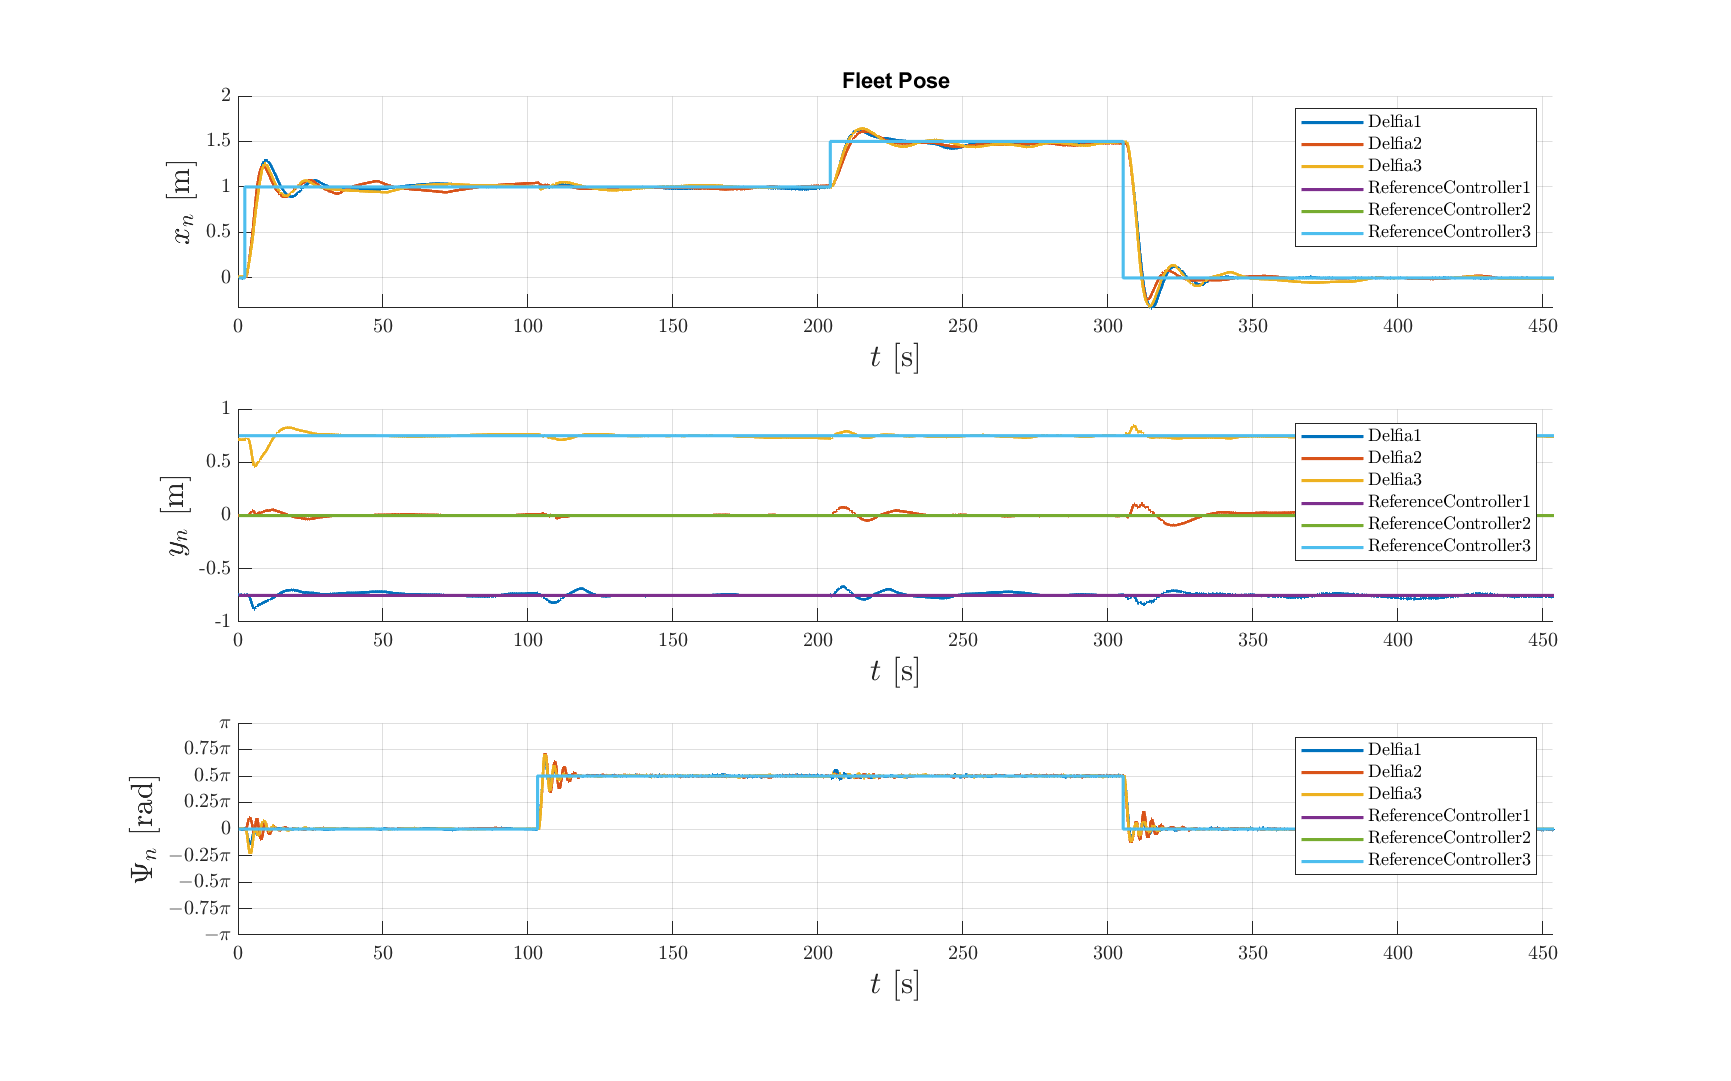
\includegraphics[width=1.0\textwidth]{matlabEvaluationFig18a.eps}
	\caption{3 separate vessels doing the similar step responses, but at an y-offset, such that they are besides oneanother. Three different step responses are done in this test representing forward, rotational and sideways motion.}
	\label{stepXYYAW1example}
\end{figure}

Throughout the process of iteratively improving control performance by adjusting gains, various insights were gained. 
A steady state error for all step responses was neglectably small without utilizing any integral control. This can be explained by the fact that the test setup was in a lab setting with little to no disturbances such as wind, current or waves. Thus there was no nessecity of setting any integral gain.
Dampening that was naturally present on the vessels proved to be quite significant without addition of derivative control. This is obviously thanks to hydrodynamic dampening. Enough dampening was considered to be naturally present in translation, and addition of more dampening terms only decreased performance. However, rotational motion did benefit from derivative control, as way more oscillation could be noticed in the responses. Magnitude of derivative gain for rotational motion formed as a balance between rise-time and settling-time. 

Hence the control gain tuning process formed control gains from the reference configuration. Following the control-gain scaling approach as described in section \ref{controlEffortGenerationDesign}, the configuration-independent control gains were set as follows
\begin{table}[H]
	\centering
\begin{tabular}{llll}
Dimention & Proportional gain & Integrator gain & Derivative gain \\
	\hline & & & \\[-5pt]
	translation $x$ and $y$ 	& $1.0$ $[m^{-1}]$		& $0$ $[s*m^{-1}]$ &  $0$  $[s^{-1}m^{-1}]$\\[3pt] 
	rotation $\Psi$ 			& $0.4456$ $[rad^{-1}]$			& $0$ $[s*rad^{-1}]$ & $0.15$ $[s^{-1}rad^{-1}]$\\ 
	\hline 
\end{tabular}
\caption{Configuration independent control gains that resulted from iterative system response evaluation and tuning.}
\end{table}

%\subsubsection{Adjustments on the assembly protocol}
The initial assembly protocol has been slightly adjusted throughout initial experiments. Early tests on platform assembly proved unable to perform within a reasonable timeframe. This was caused due to the fact that the magnet connectors did not reliably come into the area of acceptance upon which they would connect. Magnets seemed an attractive solution to connecting, especially as there was not a required approach direction during connecting, but vessels simply had to be adequately close to oneanother. Practically, modules would indeed be positioned in assembly orientation, yet oscillate a little, and not properly coming into contact. The area of acceptance proved too small for timely assembly with the current approach. The difficulties during connecting are visible in one test in particular, for which the module references and responses are shown in figure \ref{tp8_connecting_overall}. During this test the assembly protocol ran as described in section \ref{assemblyProtocolDesign} and illustrated in figure \ref{fig:matlabEvaluationFig14c}.

\begin{figure}[H]
	\centering
	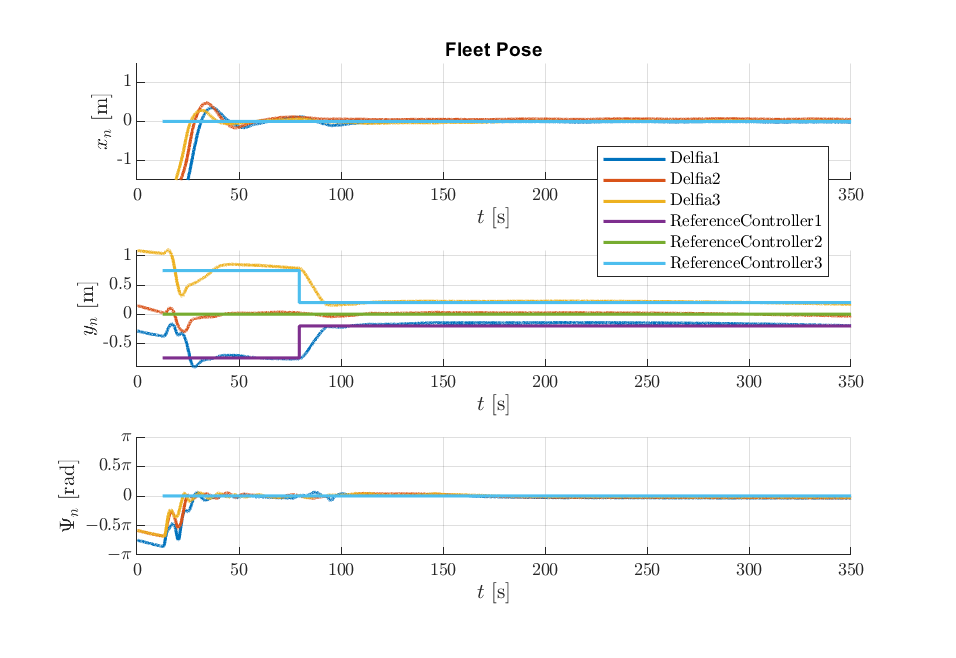
\includegraphics[width=1.0\textwidth]{tp8_connecting_overallb.eps}
	\caption{System responses during early connecting protocol. Notice how $x$ and $yaw$ reference remains constant. Most notably is the change in $y$ reference at $t=80s$. Assembly preparation and initial line-up occurs until this moment, after which the reference changes such that the vessels move to connection position.}
	\label{tp8_connecting_overall}
\end{figure}

From approximately $t=100$ one would expect modules to be approximately lined up such that magnet connectors could properly function. Successful connection can be judged in a more quantitative manner by expressing relative motion between modules. Succesful connections between modules should display zero or near zero relative motion. Figure \ref{tp8_connecting_relative_wide} \ref{AsseblyFailedRelative} show relative position between modules. For this, the body fixed frame of the middle vessel (module 2) is used, in which position of the connecting vessels (1 \& 3) are expressed (see figure \ref{fig:localframeShowing} for an illustration on how to interpret expressing location of a module in another vessel's body fixed coordinate system). 

\begin{figure}[H]
	\centering
	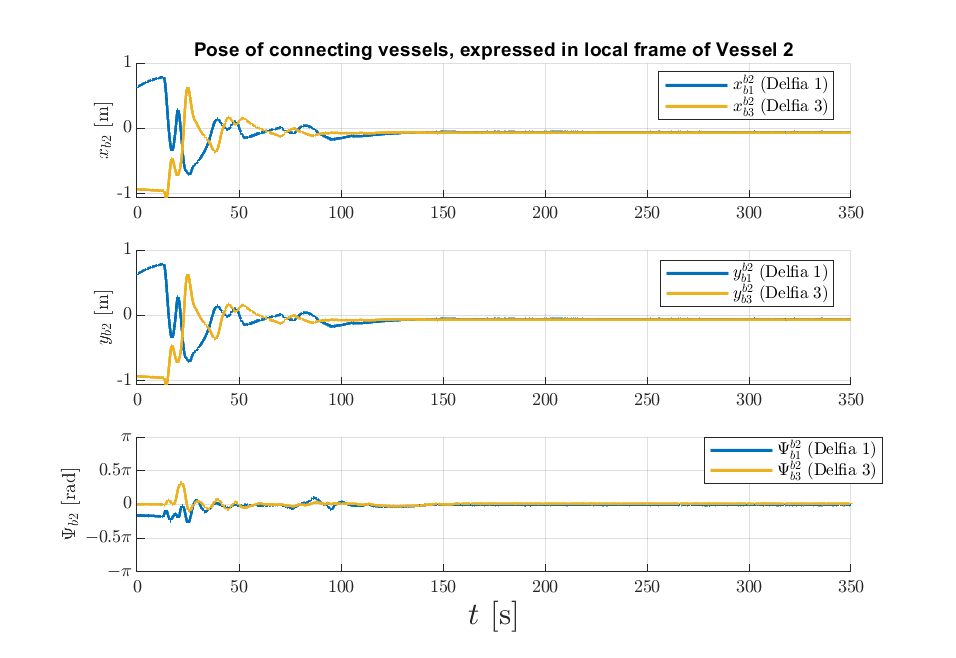
\includegraphics[width=0.9\textwidth]{tp8_connecting_relative_wide.eps}
	\caption{Relative motion of two modules connecting to module nr. 2, while running early assembly protocols.}
	\label{tp8_connecting_relative_wide}
\end{figure}

\begin{figure}[H]
	\centering
	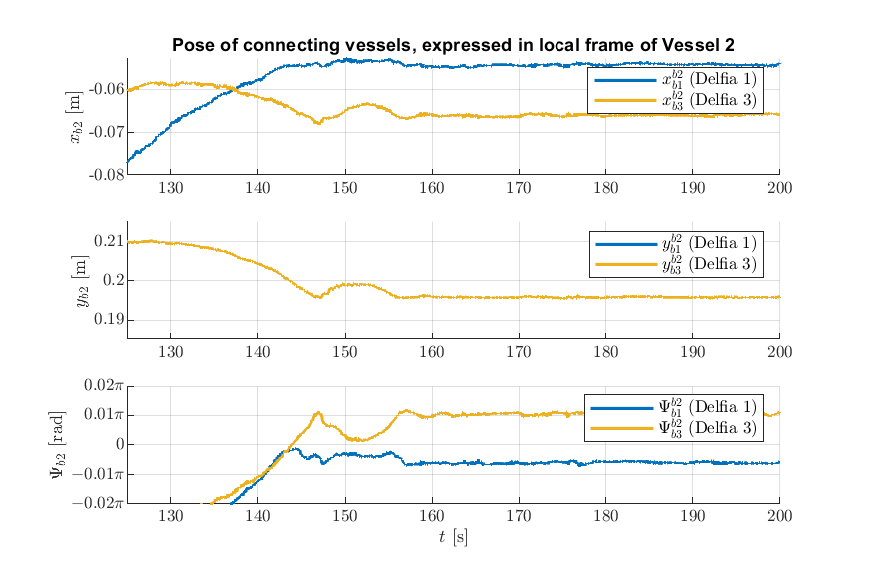
\includegraphics[width=0.9\textwidth]{tp8_connecting_relative_Zoomed.eps}
	\caption{Relative motion of two modules connecting to module nr. 2, while running early assembly protocols. Relative motion of a module stops in all three degrees of freedom, more or less at the same time, indicating succesful connection.}
	\label{AsseblyFailedRelative}
\end{figure}

Although connection was succesfully achieved, it required a period in the order of 70 seconds, which was considered rather long, even for a proof of concept. It was observed that modules were positioned near the connection site, but with lacking stimulants to get connectors into area of acceptance. Figure \ref{tp8_connecting_relative_state130t} illustrates how modules float around the connection site, while they were unconstrained in three degrees of motion, resulting in discrepancy in x y and yaw positioning.  Small errors in the definition of the body-fixed frame of the modules obtained from the optical tracking system, can be seen in figure \ref{AsseblyFailedRelative} and \ref{tp8_connecting_relative_state130t}, as the former shows nonzero $x$ and $\Psi$ values after connecting and the latter shows a seeming overlap of vessels. Relative motion in three degrees of freedom are present, which causes the modules to be misaligned, making succesful connecting less probable. Seeming overlap of module 1 \& 2 is caused by small errors in the definition of modules' origins. The definitions of the module's origins with respect to the optical trackers were slightly adjusted to decrease the magnitude of these errors for further tests. 

\begin{figure}[H]
	\centering
	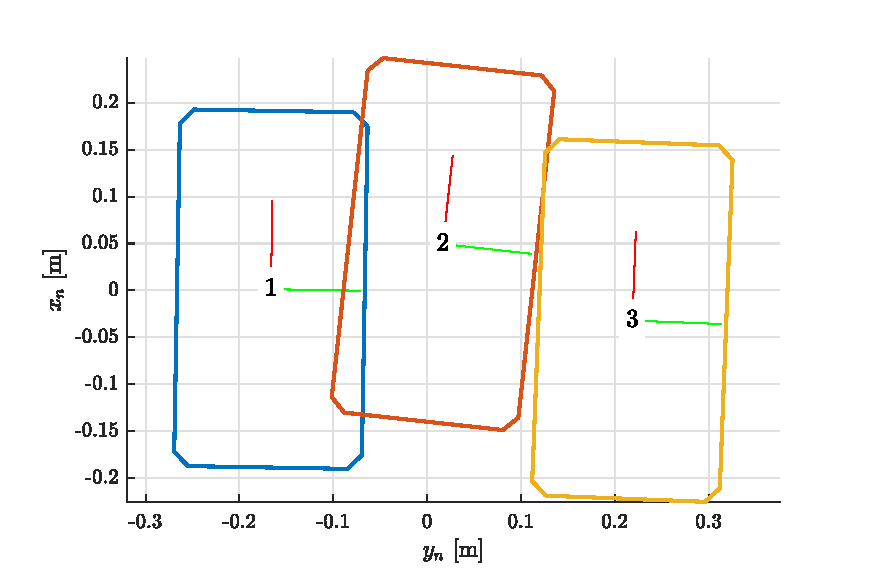
\includegraphics[width=0.7\textwidth]{tp8_connecting_relative_state130t.eps}
	\caption{Measured system state at $t=130s$ during early assembly test shown in figure \ref{tp8_connecting_relative_wide} and \ref{AsseblyFailedRelative}.}
	\label{tp8_connecting_relative_state130t}
\end{figure}
The problem of being insufficiently able to position modules within connector area of acceptance was solved by using normal forces on the modules' hulls to align surfaces. This is a common trick used by regular, human operated ships. A characteristic example is a ferry that pushes itself to a dock, such that it does not rotate or move, allowing safe transfer of passengers. A small normal force between vessels ensures that they keep making contact, and avoid rotation. As modules made contact, only one motion remained, which was translation along the contact surface. With only one degree of (relative) motion connections could be made timely. Figure \ref{DelfiasNormalForceIntoPush2} shows how normal forces have been created by setting contoller reference somewhat within the rigid body of a neighbouring module. Figure \ref{tp8_connecting_relative_wide} shows relative motion between modules of an assembling system that apply this approach. Notice that relative rotation and motion perpendicular to the contact surface are constrained first. Sliding motion along contact surface later stops as connectors snap into place. 

 \begin{figure}[H]
	\centering
	\makebox[\textwidth][c]{
		\begin{minipage}{0.47\textwidth}
			\centering
			\includegraphics[width=1\textwidth]{img/3x1ConfigurationRef}
			\caption{Initial reference positions of modules for assembly}
			\label{3x1ConfigurationRef}
		\end{minipage}\hfill
		\begin{minipage}{0.45\textwidth}
			\centering
			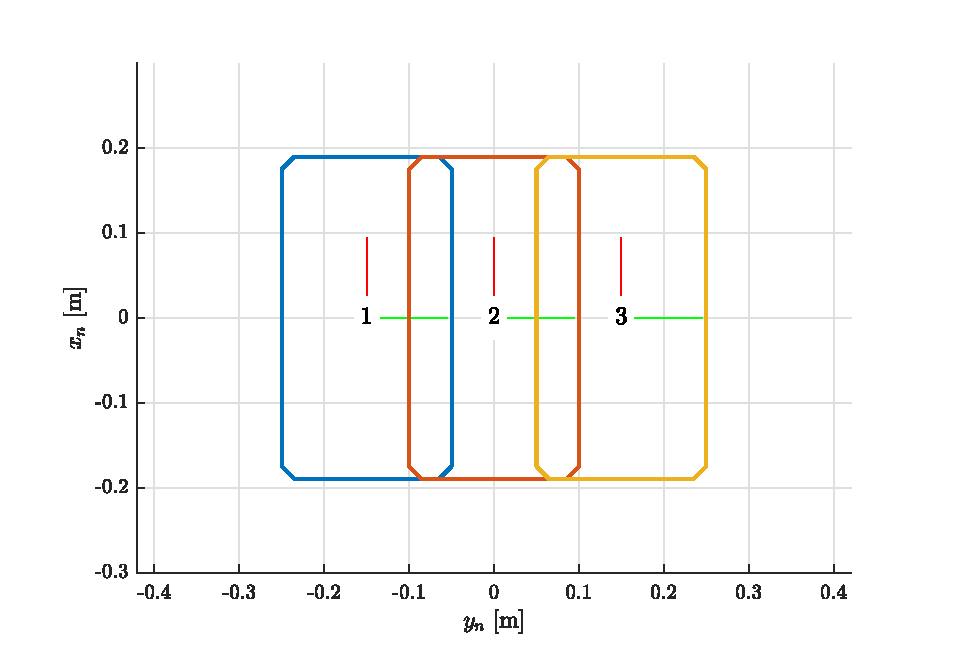
\includegraphics[width=1\textwidth]{img/3x1ConfigurationRef_overlapping}
			\caption{Adjusted references for positioning of modules while connecting, to create some normal forces between hulls. The shown references are impossible for the system to reach, as vessels are constrained by their hulls which can not overlap.}
			\label{3x1ConfigurationRef_overlapping}
		\end{minipage}
	}
\end{figure}

\begin{figure}[H]
	\centering
	\includegraphics[width=0.4\textwidth]{VesselConnectTopvieuwReference_early.eps}
	\caption{Normal forces that result from overlapping references during assembly.}
	\label{DelfiasNormalForceIntoPush2}
\end{figure}

The normal forces between modules were kept to a minimum, as they purely function to remove motion between vessels perpendicular to the connection surface ($y$), and rotation. Remaining motion was by sliding along the connecting surface of the hull ($x$ direction), where friction did not seem to play a significant role with a smooth surface and low normal forces. 



\vspace{15mm}

This chapter explained design choices that characterize the developed self-assembling and cooperative fleet control system. At first, the multi-robot control approach with variable topology is explained after which the design of each subsystem is discussed. Implementation is thereafter explained, showing the realization of the fleet control system. The next chapter will assess performance of the  developed framework, to see whether or not the system performs according to the presented design criteria and goals. 

